% Options for packages loaded elsewhere
% Options for packages loaded elsewhere
\PassOptionsToPackage{unicode}{hyperref}
\PassOptionsToPackage{hyphens}{url}
\PassOptionsToPackage{dvipsnames,svgnames,x11names}{xcolor}
%
\documentclass[
  letterpaper,
  DIV=11,
  numbers=noendperiod]{scrartcl}
\usepackage{xcolor}
\usepackage{amsmath,amssymb}
\setcounter{secnumdepth}{-\maxdimen} % remove section numbering
\usepackage{iftex}
\ifPDFTeX
  \usepackage[T1]{fontenc}
  \usepackage[utf8]{inputenc}
  \usepackage{textcomp} % provide euro and other symbols
\else % if luatex or xetex
  \usepackage{unicode-math} % this also loads fontspec
  \defaultfontfeatures{Scale=MatchLowercase}
  \defaultfontfeatures[\rmfamily]{Ligatures=TeX,Scale=1}
\fi
\usepackage{lmodern}
\ifPDFTeX\else
  % xetex/luatex font selection
\fi
% Use upquote if available, for straight quotes in verbatim environments
\IfFileExists{upquote.sty}{\usepackage{upquote}}{}
\IfFileExists{microtype.sty}{% use microtype if available
  \usepackage[]{microtype}
  \UseMicrotypeSet[protrusion]{basicmath} % disable protrusion for tt fonts
}{}
\makeatletter
\@ifundefined{KOMAClassName}{% if non-KOMA class
  \IfFileExists{parskip.sty}{%
    \usepackage{parskip}
  }{% else
    \setlength{\parindent}{0pt}
    \setlength{\parskip}{6pt plus 2pt minus 1pt}}
}{% if KOMA class
  \KOMAoptions{parskip=half}}
\makeatother
% Make \paragraph and \subparagraph free-standing
\makeatletter
\ifx\paragraph\undefined\else
  \let\oldparagraph\paragraph
  \renewcommand{\paragraph}{
    \@ifstar
      \xxxParagraphStar
      \xxxParagraphNoStar
  }
  \newcommand{\xxxParagraphStar}[1]{\oldparagraph*{#1}\mbox{}}
  \newcommand{\xxxParagraphNoStar}[1]{\oldparagraph{#1}\mbox{}}
\fi
\ifx\subparagraph\undefined\else
  \let\oldsubparagraph\subparagraph
  \renewcommand{\subparagraph}{
    \@ifstar
      \xxxSubParagraphStar
      \xxxSubParagraphNoStar
  }
  \newcommand{\xxxSubParagraphStar}[1]{\oldsubparagraph*{#1}\mbox{}}
  \newcommand{\xxxSubParagraphNoStar}[1]{\oldsubparagraph{#1}\mbox{}}
\fi
\makeatother


\usepackage{longtable,booktabs,array}
\newcounter{none} % for unnumbered tables
\usepackage{calc} % for calculating minipage widths
% Correct order of tables after \paragraph or \subparagraph
\usepackage{etoolbox}
\makeatletter
\patchcmd\longtable{\par}{\if@noskipsec\mbox{}\fi\par}{}{}
\makeatother
% Allow footnotes in longtable head/foot
\IfFileExists{footnotehyper.sty}{\usepackage{footnotehyper}}{\usepackage{footnote}}
\makesavenoteenv{longtable}
\usepackage{graphicx}
\makeatletter
\newsavebox\pandoc@box
\newcommand*\pandocbounded[1]{% scales image to fit in text height/width
  \sbox\pandoc@box{#1}%
  \Gscale@div\@tempa{\textheight}{\dimexpr\ht\pandoc@box+\dp\pandoc@box\relax}%
  \Gscale@div\@tempb{\linewidth}{\wd\pandoc@box}%
  \ifdim\@tempb\p@<\@tempa\p@\let\@tempa\@tempb\fi% select the smaller of both
  \ifdim\@tempa\p@<\p@\scalebox{\@tempa}{\usebox\pandoc@box}%
  \else\usebox{\pandoc@box}%
  \fi%
}
% Set default figure placement to htbp
\def\fps@figure{htbp}
\makeatother





\setlength{\emergencystretch}{3em} % prevent overfull lines

\providecommand{\tightlist}{%
  \setlength{\itemsep}{0pt}\setlength{\parskip}{0pt}}



 


\KOMAoption{captions}{tableheading}
\makeatletter
\@ifpackageloaded{tcolorbox}{}{\usepackage[skins,breakable]{tcolorbox}}
\@ifpackageloaded{fontawesome5}{}{\usepackage{fontawesome5}}
\definecolor{quarto-callout-color}{HTML}{909090}
\definecolor{quarto-callout-note-color}{HTML}{0758E5}
\definecolor{quarto-callout-important-color}{HTML}{CC1914}
\definecolor{quarto-callout-warning-color}{HTML}{EB9113}
\definecolor{quarto-callout-tip-color}{HTML}{00A047}
\definecolor{quarto-callout-caution-color}{HTML}{FC5300}
\definecolor{quarto-callout-color-frame}{HTML}{acacac}
\definecolor{quarto-callout-note-color-frame}{HTML}{4582ec}
\definecolor{quarto-callout-important-color-frame}{HTML}{d9534f}
\definecolor{quarto-callout-warning-color-frame}{HTML}{f0ad4e}
\definecolor{quarto-callout-tip-color-frame}{HTML}{02b875}
\definecolor{quarto-callout-caution-color-frame}{HTML}{fd7e14}
\makeatother
\makeatletter
\@ifpackageloaded{caption}{}{\usepackage{caption}}
\AtBeginDocument{%
\ifdefined\contentsname
  \renewcommand*\contentsname{Table of contents}
\else
  \newcommand\contentsname{Table of contents}
\fi
\ifdefined\listfigurename
  \renewcommand*\listfigurename{List of Figures}
\else
  \newcommand\listfigurename{List of Figures}
\fi
\ifdefined\listtablename
  \renewcommand*\listtablename{List of Tables}
\else
  \newcommand\listtablename{List of Tables}
\fi
\ifdefined\figurename
  \renewcommand*\figurename{Figure}
\else
  \newcommand\figurename{Figure}
\fi
\ifdefined\tablename
  \renewcommand*\tablename{Table}
\else
  \newcommand\tablename{Table}
\fi
}
\@ifpackageloaded{float}{}{\usepackage{float}}
\floatstyle{ruled}
\@ifundefined{c@chapter}{\newfloat{codelisting}{h}{lop}}{\newfloat{codelisting}{h}{lop}[chapter]}
\floatname{codelisting}{Listing}
\newcommand*\listoflistings{\listof{codelisting}{List of Listings}}
\makeatother
\makeatletter
\makeatother
\makeatletter
\@ifpackageloaded{caption}{}{\usepackage{caption}}
\@ifpackageloaded{subcaption}{}{\usepackage{subcaption}}
\makeatother
\usepackage{bookmark}
\IfFileExists{xurl.sty}{\usepackage{xurl}}{} % add URL line breaks if available
\urlstyle{same}
% fallback for those not using the hyperref driver hyperxmp:
\makeatletter
\@ifundefined{xmpquote}{\newcommand{\xmpquote}[1]{#1}}{}
\makeatother
\hypersetup{
  pdftitle={Terrorist Targeting{,} Relative Capacity{,} and State Military Response},
  pdfauthor={Author Name},
  colorlinks=true,
  linkcolor={blue},
  filecolor={Maroon},
  citecolor={Blue},
  urlcolor={Blue},
  pdfcreator={LaTeX via pandoc}}


\title{Terrorist Targeting, Relative Capacity, and State Military
Response}
\author{Author Name}
\date{2026-11-20}
\begin{document}
\maketitle

\renewcommand*\contentsname{Table of contents}
{
\setcounter{tocdepth}{3}
\tableofcontents
}

\section{Theoretical Objective}\label{theoretical-objective}

Why do some terrorist campaigns remain matters for police and
intelligence agencies, while others induce governments to employ
military force? This section develops a parsimonious
incomplete-information game in which terrorist targeting affects state
response through two mechanisms.

First, targeting creates \textbf{regime-specific political pressure}.
Civilian attacks are especially consequential for democratic governments
because elected officials are accountable to a broad public. Security
attacks are especially consequential for autocratic governments because
the military, police, and intelligence services constitute central
pillars of regime survival.

Second, targeting provides \textbf{information about terrorist
capacity}. Sustaining attacks against state security institutions is
more characteristic of high-capacity terrorist organizations than of
low-capacity organizations. Repeated security attacks therefore cause
the government to revise upward its estimate of terrorist capacity.

Whether these pressures result in military action depends on the
terrorist organization's inferred capacity \textbf{relative to the
government's counterterrorism capacity}. A capable state can address a
wider range of terrorist threats through police and intelligence
instruments. A less capable state is more likely to confront a terrorist
threat that exceeds what its internal-security institutions can manage.

The model's central logic is:

\[
\boxed{
\text{Targeting frequencies}
\longrightarrow
\begin{cases}
\text{regime-specific political pressure},\\
\text{inferred terrorist capacity}
\end{cases}
\longrightarrow
\text{relative threat}
\longrightarrow
\{P,M\}.
}
\]

Here, \(P\) denotes intensified police and internal-security measures,
while \(M\) denotes military mobilization or deployment.

\section{Players, Types, and Sequence of
Play}\label{players-types-and-sequence-of-play}

\subsection{Terrorist capacity}\label{terrorist-capacity}

Consider a Bayesian game between a terrorist organization \(T\) and a
government \(G\). The terrorist organization has privately known
organizational capacity:

\[
\theta\in\{\theta_L,\theta_H\},
\qquad
0<\theta_L<\theta_H.
\]

The organization observes its own type, but the government does not. The
government's prior probability that it confronts a high-capacity
organization is:

\[
\Pr(\theta=\theta_H)=\pi_0,
\qquad
0<\pi_0<1.
\]

High capacity may reflect personnel, recruitment networks, intelligence
and reconnaissance, logistics, weapons access, command and control,
evasion of state surveillance, and the ability to replace operatives and
sustain attacks over time. The government need not observe these
attributes separately. It instead infers \(\theta\) from the
organization's observable targeting behavior.

\subsection{Government capacity}\label{government-capacity}

Let:

\[
g>0
\]

denote the government's relevant counterterrorism capacity. This
includes the capabilities of police, intelligence, judicial,
border-control, and related internal-security institutions. The
government knows its own capacity. For parsimony, \(g\) is also
observable to the terrorist organization.

Government capacity matters because the security consequences of
terrorist capacity depend on the state's ability to contain the threat.
The same terrorist organization constitutes a more serious relative
threat to a state with weak police and intelligence institutions than to
a state with extensive surveillance, investigative, and enforcement
capabilities.

\subsection{Targeting outcomes}\label{targeting-outcomes}

During the period under observation, the terrorist campaign produces:

\[
\mathbf n=(n_C,n_S),
\]

where \(n_C\) is the frequency of attacks against civilian targets and
\(n_S\) is the frequency of attacks against state security targets.
Security targets include military personnel and facilities, police,
intelligence agencies, and other coercive institutions.

These variables measure \textbf{target-specific campaign intensity}, not
attack severity. One large attack and many smaller attacks may produce
different values of \((n_C,n_S)\) even when their total casualties are
similar.

\subsection{Government response}\label{government-response}

After observing \(\mathbf n\), the government chooses:

\[
r\in\{P,M\},
\]

where \(P\) denotes intensified policing, intelligence, judicial, or
other internal-security measures and \(M\) denotes mobilization or
deployment of military forces. The model focuses on the choice between
these two escalatory instruments and therefore takes as given that the
government has already chosen to respond more forcefully than under the
preexisting status quo.

\subsection{Sequence of play}\label{sequence-of-play}

The sequence is:

\begin{enumerate}
\def\labelenumi{\arabic{enumi}.}
\tightlist
\item
  Nature draws terrorist capacity \(\theta\).
\item
  The terrorist organization observes \(\theta\) and selects a targeting
  strategy.
\item
  Civilian and security attack frequencies \((n_C,n_S)\) are realized
  stochastically.
\item
  The government observes \((n_C,n_S)\) but not \(\theta\).
\item
  The government updates its belief about \(\theta\).
\item
  The government evaluates inferred terrorist capacity relative to
  government capacity \(g\).
\item
  The government chooses \(P\) or \(M\).
\end{enumerate}

In compact form:

\[
\boxed{
\theta
\longrightarrow
(\lambda_C,\lambda_S)
\longrightarrow
(n_C,n_S)
\longrightarrow
\mu(n_C,n_S)
\longrightarrow
\widehat{\rho}(n_C,n_S,g)
\longrightarrow
r\in\{P,M\}.
}
\]

\section{Extensive-Form
Representation}\label{extensive-form-representation}

The game is represented in Figure~\ref{fig-game-tree}. Nature first
draws terrorist capacity. Each terrorist type chooses target-specific
campaign rates. These choices generate stochastic attack frequencies.
The government observes the realized frequencies but not terrorist type,
updates its belief, computes the expected terrorist-government
capability ratio, and chooses between policing and military force.

\begin{figure}

\centering{

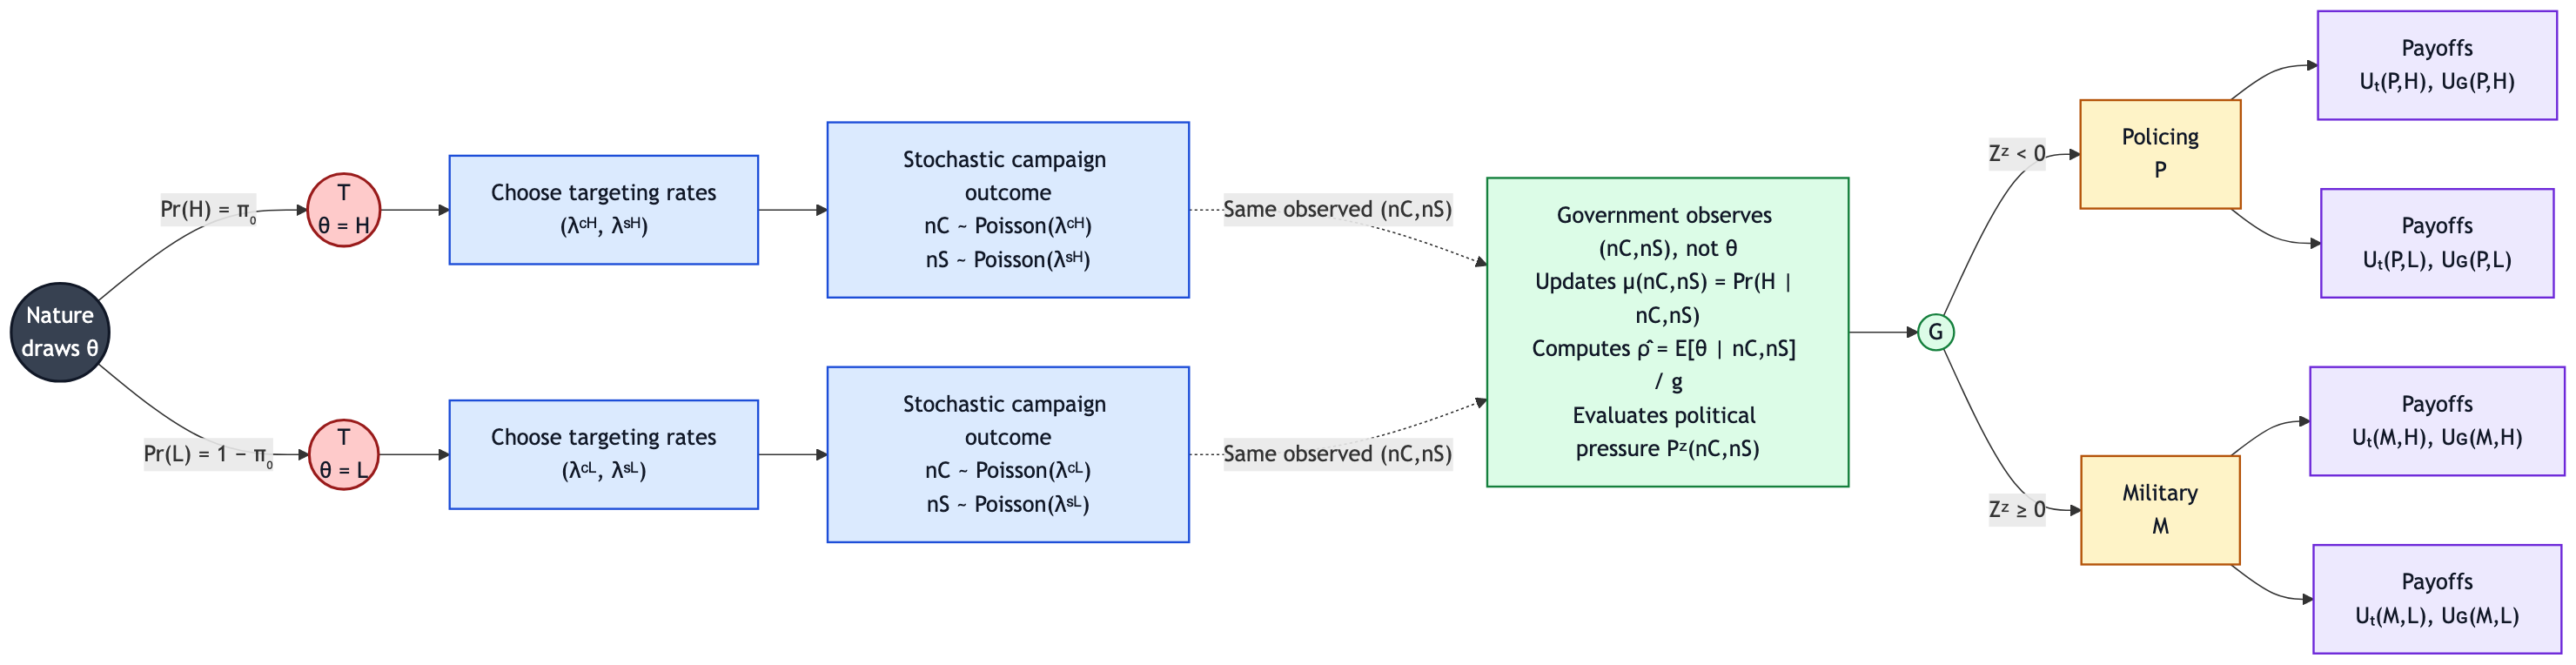
\includegraphics[width=19.3in,height=4.98in]{Download the complete Quarto file_files/figure-latex/mermaid-figure-1.png}

}

\caption{\label{fig-game-tree}Extensive-form representation of terrorist
targeting, Bayesian updating, relative capacity, and state response.}

\end{figure}%

The dashed branches in Figure~\ref{fig-game-tree} represent the
government's informational problem. Histories generated by different
terrorist types belong to the same information set whenever they produce
the same observed count vector \((n_C,n_S)\). The government knows the
campaign it observed, but not the type that generated it.

\section{Terrorist Targeting and Stochastic Attack
Frequencies}\label{terrorist-targeting-and-stochastic-attack-frequencies}

The terrorist organization selects a campaign strategy:

\[
\boldsymbol{\lambda}=(\lambda_C,\lambda_S),
\]

where \(\lambda_C\) and \(\lambda_S\) are intended rates of civilian and
security attacks. The strategy may depend on terrorist capacity,
government capacity, and regime type:

\[
\boldsymbol{\lambda}^*(\theta,g,z)
=
\left(
\lambda_C^*(\theta,g,z),
\lambda_S^*(\theta,g,z)
\right),
\]

where \(z\in\{D,A\}\) denotes democracy or autocracy.

Realized attack frequencies are stochastic. Assume:

\[
n_C\mid\theta\sim\operatorname{Poisson}(\lambda_C^\theta)
\]

and:

\[
n_S\mid\theta\sim\operatorname{Poisson}(\lambda_S^\theta).
\]

This formulation separates the organization's intended campaign from
realized outcomes. Even after selecting attack rates, the organization
does not perfectly control how many operations occur. Attacks may be
prevented, disrupted, delayed, or abandoned.

For analytical simplicity, civilian and security attack counts are
conditionally independent given terrorist type:

\[
\Pr(n_C,n_S\mid\theta)
=
\Pr(n_C\mid\theta)\Pr(n_S\mid\theta).
\]

Thus:

\[
\Pr(n_C,n_S\mid\theta)
=
\frac{e^{-\lambda_C^\theta}(\lambda_C^\theta)^{n_C}}{n_C!}
\frac{e^{-\lambda_S^\theta}(\lambda_S^\theta)^{n_S}}{n_S!}.
\tag{1}
\]

\section{Informational Assumption}\label{informational-assumption}

The model requires one principal assumption about terrorist behavior:

\[
\boxed{
\frac{\lambda_S^H}{\lambda_S^L}
>
\frac{\lambda_C^H}{\lambda_C^L}.
}
\tag{A1}
\]

The relative frequency of security targeting differs more strongly
between high- and low-capacity organizations than does the relative
frequency of civilian targeting.

A particularly parsimonious baseline assumes:

\[
\lambda_C^H=\lambda_C^L
\tag{A1a}
\]

and:

\[
\lambda_S^H>\lambda_S^L.
\tag{A1b}
\]

Under these assumptions, civilian attack frequency provides no direct
information about whether the organization is high or low capacity,
while security attack frequency is positively informative. This does not
imply that civilian attacks are unimportant. Their effect operates
principally through political pressure rather than through the
government's capacity assessment.

The assumption concerns campaign persistence rather than hardness of
individual targets. A low-capacity organization may occasionally attack
a police officer or patrol. Sustaining a larger number of attacks
against state security institutions, however, is more characteristic of
a high-capacity organization.

\section{Bayesian Updating}\label{bayesian-updating}

After observing \((n_C,n_S)\), the government calculates the posterior
probability that the organization is high capacity:

\[
\mu(n_C,n_S)
=
\Pr(\theta=\theta_H\mid n_C,n_S).
\]

Bayes' rule gives:

\[
\boxed{
\mu(n_C,n_S)
=
\frac{\pi_0 f_H(n_C,n_S)}
{\pi_0 f_H(n_C,n_S)+(1-\pi_0)f_L(n_C,n_S)},
}
\tag{2}
\]

where \(f_\theta(n_C,n_S)=\Pr(n_C,n_S\mid\theta)\).

\subsection{Posterior odds}\label{posterior-odds}

Define prior odds as:

\[
\Omega_0=\frac{\pi_0}{1-\pi_0}.
\]

Posterior odds are:

\[
\Omega(n_C,n_S)
=
\frac{\mu(n_C,n_S)}{1-\mu(n_C,n_S)}
=
\Omega_0\frac{f_H(n_C,n_S)}{f_L(n_C,n_S)}.
\]

Substituting the Poisson probabilities yields:

\[
\boxed{
\begin{aligned}
\Omega(n_C,n_S)
={}&\Omega_0
\exp\left[-(\lambda_C^H-\lambda_C^L)-(\lambda_S^H-\lambda_S^L)\right]\\
&\times
\left(\frac{\lambda_C^H}{\lambda_C^L}\right)^{n_C}
\left(\frac{\lambda_S^H}{\lambda_S^L}\right)^{n_S}.
\end{aligned}
}
\tag{3}
\]

Taking logarithms makes the informational content of each attack
frequency transparent:

\[
\boxed{
\begin{aligned}
\log\Omega(n_C,n_S)
={}&\log\Omega_0
-(\lambda_C^H-\lambda_C^L)
-(\lambda_S^H-\lambda_S^L)\\
&+n_C\log\left(\frac{\lambda_C^H}{\lambda_C^L}\right)
+n_S\log\left(\frac{\lambda_S^H}{\lambda_S^L}\right).
\end{aligned}
}
\tag{4}
\]

An additional civilian attack changes posterior log-odds by:

\[
\frac{\partial\log\Omega}{\partial n_C}
=
\log\left(\frac{\lambda_C^H}{\lambda_C^L}\right),
\tag{5}
\]

while an additional security attack changes posterior log-odds by:

\[
\frac{\partial\log\Omega}{\partial n_S}
=
\log\left(\frac{\lambda_S^H}{\lambda_S^L}\right).
\tag{6}
\]

Under Assumption A1:

\[
\boxed{
\frac{\partial\log\Omega}{\partial n_S}
>
\frac{\partial\log\Omega}{\partial n_C}.
}
\tag{7}
\]

Under the baseline assumption \(\lambda_C^H=\lambda_C^L\):

\[
\frac{\partial\mu}{\partial n_C}=0,
\qquad
\frac{\partial\mu}{\partial n_S}>0.
\tag{8}
\]

Civilian attacks therefore affect response through political pressure,
whereas security attacks affect response through both information and
political pressure.

\section{Inferred Terrorist-Government Relative
Capacity}\label{inferred-terrorist-government-relative-capacity}

The government responds not to terrorist capacity in isolation, but to
terrorist capacity relative to its own ability to contain the threat.
Define expected relative capacity as:

\[
\boxed{
\widehat{\rho}(n_C,n_S,g)
=
\frac{E[\theta\mid n_C,n_S]}{g}.
}
\tag{9}
\]

Because terrorist capacity has two possible values:

\[
E[\theta\mid n_C,n_S]
=
\mu(n_C,n_S)\theta_H
+[1-\mu(n_C,n_S)]\theta_L.
\]

Therefore:

\[
\boxed{
\widehat{\rho}(n_C,n_S,g)
=
\frac{\mu(n_C,n_S)\theta_H+[1-\mu(n_C,n_S)]\theta_L}{g}.
}
\tag{10}
\]

A higher posterior probability of confronting a high-capacity
organization increases relative threat:

\[
\frac{\partial\widehat{\rho}}{\partial\mu}
=
\frac{\theta_H-\theta_L}{g}>0.
\tag{11}
\]

Greater government capacity reduces relative threat:

\[
\boxed{
\frac{\partial\widehat{\rho}}{\partial g}
=
-\frac{\mu\theta_H+(1-\mu)\theta_L}{g^2}<0.
}
\tag{12}
\]

Under the informational assumptions:

\[
\frac{\partial\widehat{\rho}}{\partial n_S}
=
\frac{\theta_H-\theta_L}{g}
\frac{\partial\mu}{\partial n_S}>0.
\tag{13}
\]

Moreover:

\[
\boxed{
\frac{\partial^2\widehat{\rho}}
{\partial n_S\partial g}
=
-\frac{\theta_H-\theta_L}{g^2}
\frac{\partial\mu}{\partial n_S}<0.
}
\tag{14}
\]

The increase in relative threat produced by an additional informative
security attack is therefore smaller for governments with greater
counterterrorism capacity.

\section{Regime-Specific Political
Pressure}\label{regime-specific-political-pressure}

Let political pressure be:

\[
P^z(n_C,n_S)
=
\alpha_C^z n_C+\alpha_S^z n_S,
\tag{15}
\]

where \(\alpha_C^z\) is the political pressure generated by an
additional civilian attack and \(\alpha_S^z\) is the pressure generated
by an additional security attack.

\subsection{Democracies}\label{democracies}

For democracies:

\[
\boxed{
\alpha_C^D>\alpha_S^D>0.
}
\tag{A2}
\]

Civilian attacks are particularly consequential because elected leaders
are accountable to a broad public. Repeated attacks on civilians can
generate electoral punishment, media scrutiny, opposition criticism, and
demands for stronger action. Security attacks also impose political
costs, but their direct public-accountability effect is smaller.

\subsection{Autocracies}\label{autocracies}

For autocracies:

\[
\boxed{
\alpha_S^A>\alpha_C^A\geq0.
}
\tag{A3}
\]

Security attacks are particularly consequential because military,
police, and intelligence institutions are central to regime protection.
Repeated attacks on these institutions can expose weakness, damage
regime prestige, undermine coercive control, or encourage challengers.

\subsection{Cross-regime comparisons}\label{cross-regime-comparisons}

To derive the intended two-by-two comparison, assume:

\[
\boxed{\alpha_C^D>\alpha_C^A}
\tag{A4}
\]

and:

\[
\boxed{\alpha_S^A>\alpha_S^D.}
\tag{A5}
\]

Civilian attacks therefore create greater direct political pressure in
democracies, while security attacks create greater direct political
pressure in autocracies. These assumptions concern the political channel
only. The informational content of security attacks applies across both
regime types.

\section{Government Choice Between Policing and Military
Action}\label{government-choice-between-policing-and-military-action}

Let expected government loss from response \(r\) be:

\[
L_G(r)
=
K_r+l_rP^z(n_C,n_S)+D(r,\widehat{\rho}),
\tag{16}
\]

where \(K_r\) is the direct cost of response, \(l_r\) is the proportion
of political pressure remaining after the response, and
\(D(r,\widehat{\rho})\) is expected future security loss.

Assume:

\[
K_M>K_P
\tag{A6}
\]

because military action requires greater fiscal, administrative,
logistical, and political commitment. Also assume:

\[
l_M<l_P.
\tag{A7}
\]

Military action provides a stronger demonstration of resolve and
therefore alleviates more political pressure than policing alone.

Define:

\[
\Delta K=K_M-K_P>0
\]

and:

\[
\Delta l=l_P-l_M>0.
\]

Finally, assume the additional security benefit of military action is
increasing in relative threat:

\[
D(P,\widehat{\rho})-D(M,\widehat{\rho})
=
\delta\widehat{\rho},
\qquad
\delta>0.
\tag{17}
\]

Military action provides a larger advantage over policing when the
terrorist organization is more capable relative to the government.

\subsection{Military-response
condition}\label{military-response-condition}

The government chooses \(M\) when \(L_G(M)\leq L_G(P)\). Rearranging
gives:

\[
\boxed{
P^z(n_C,n_S)\Delta l
+\delta\widehat{\rho}(n_C,n_S,g)
\geq
\Delta K.
}
\tag{18}
\]

The left side contains the benefits of military escalation. The first
term is the additional political pressure relieved by military action.
The second is the additional security benefit of military action against
a relatively capable threat. The right side is the incremental cost of
using military rather than police instruments.

Define the latent net benefit of military action:

\[
\boxed{
Z^z(n_C,n_S,g)
=
P^z(n_C,n_S)\Delta l
+\delta\widehat{\rho}(n_C,n_S,g)
-\Delta K.
}
\tag{19}
\]

The government's optimal response is:

\[
\boxed{
r^*=
\begin{cases}
P, & Z^z(n_C,n_S,g)<0,\\[4pt]
M, & Z^z(n_C,n_S,g)\geq0.
\end{cases}
}
\tag{20}
\]

\section{Stochastic Government
Choice}\label{stochastic-government-choice}

Military decisions may also depend on factors unobserved by the analyst,
including budgetary constraints, international opposition, military
readiness, leadership preferences, or competing security commitments.
Introduce a response shock:

\[
\varepsilon\sim\operatorname{Logistic}(0,s).
\]

The realized net benefit of military action is:

\[
Z^{z*}=Z^z+\varepsilon.
\]

The probability of military response is:

\[
\boxed{
\Pr(M\mid n_C,n_S,g,z)
=
\Lambda\left[
\frac{P^z(n_C,n_S)\Delta l
+\delta\widehat{\rho}(n_C,n_S,g)
-\Delta K}{s}
\right],
}
\tag{21}
\]

where:

\[
\Lambda(x)=\frac{1}{1+e^{-x}}.
\]

The stochastic formulation does not change the strategic logic. It
converts the deterministic \(P\)-versus-\(M\) threshold into a
probability of observing military action.

\section{Implications of Civilian Attack
Frequency}\label{implications-of-civilian-attack-frequency}

Consider an increase in \(n_C\), holding \(n_S\) and \(g\) constant.
Differentiating the net benefit of military action gives:

\[
\frac{\partial Z^z}{\partial n_C}
=
\alpha_C^z\Delta l
+\delta\frac{\partial\widehat{\rho}}{\partial n_C}.
\tag{22}
\]

Under the baseline assumption that civilian attack frequency is
uninformative about terrorist type:

\[
\frac{\partial\widehat{\rho}}{\partial n_C}=0.
\]

Therefore:

\[
\boxed{
\frac{\partial Z^z}{\partial n_C}
=
\alpha_C^z\Delta l>0.
}
\tag{23}
\]

More civilian attacks increase the attractiveness of military action in
both regime types because they increase political pressure. The
cross-regime difference follows from \(\alpha_C^D>\alpha_C^A\):

\[
\boxed{
\frac{\partial Z^D}{\partial n_C}
>
\frac{\partial Z^A}{\partial n_C}>0.
}
\tag{24}
\]

\subsection{Democracy}\label{democracy}

In democracies:

\[
n_C\uparrow
\Rightarrow
P^D(n_C,n_S)\uparrow
\Rightarrow
Z^D\uparrow.
\]

At relatively low civilian-target frequency, the government may retain
intensified policing. Once civilian attacks generate enough pressure for
\(Z^D\geq0\), the government transitions to military action:

\[
\boxed{
n_C\uparrow:
\qquad
P\longrightarrow M
\quad\text{relatively readily in democracies}.}
\]

\subsection{Autocracy}\label{autocracy}

Civilian attacks also increase political pressure in autocracies if
\(\alpha_C^A>0\), but the increase is smaller because
\(\alpha_C^A<\alpha_C^D\). Autocratic governments therefore remain with
policing over a wider range of civilian attack frequencies and
transition to military action only after civilian attacks become
sufficiently frequent or when they are already near the military
threshold:

\[
\boxed{
n_C\uparrow:
\qquad
P\text{ persists longer before }M
\quad\text{in autocracies}.}
\]

\begin{tcolorbox}[enhanced jigsaw, arc=.35mm, bottomrule=.15mm, bottomtitle=1mm, breakable, colback=white, colbacktitle=quarto-callout-important-color!10!white, colframe=quarto-callout-important-color-frame, coltitle=black, left=2mm, leftrule=.75mm, opacityback=0, opacitybacktitle=0.6, rightrule=.15mm, title=\textcolor{quarto-callout-important-color}{\faExclamation}\hspace{0.5em}{Proposition 1: Civilian-target frequency}, titlerule=0mm, toprule=.15mm, toptitle=1mm]

Holding security targeting, government capacity, and response costs
constant, increasing civilian-target attack frequency raises the
likelihood of military response in both regimes. The increase operates
primarily through political pressure and is stronger in democracies:

\[
\frac{\partial Z^D}{\partial n_C}
>
\frac{\partial Z^A}{\partial n_C}>0.
\]

\end{tcolorbox}

\section{Implications of Security Attack
Frequency}\label{implications-of-security-attack-frequency}

Now consider an increase in \(n_S\), holding \(n_C\) and \(g\) constant.
Differentiating gives:

\[
\boxed{
\frac{\partial Z^z}{\partial n_S}
=
\alpha_S^z\Delta l
+\delta\frac{\partial\widehat{\rho}}{\partial n_S}.
}
\tag{25}
\]

Unlike civilian attack frequency, security attack frequency operates
through two mechanisms. The first term is the political-pressure effect.
The second is the informational effect. Because
\(\partial\widehat{\rho}/\partial n_S>0\):

\[
\boxed{
\frac{\partial Z^z}{\partial n_S}>0
}
\tag{26}
\]

in both regime types.

\subsection{Democracy}\label{democracy-1}

In democracies, the direct political effect of security targeting is
relatively modest because \(\alpha_S^D<\alpha_C^D\). Nevertheless,
repeated security attacks cause the government to revise upward its
estimate of terrorist capacity:

\[
n_S\uparrow
\Rightarrow
\mu(n_C,n_S)\uparrow
\Rightarrow
\widehat{\rho}(n_C,n_S,g)\uparrow
\Rightarrow
Z^D\uparrow.
\]

At low security-target frequency, the government may rely on policing.
As security targeting supplies greater evidence of a capable adversary,
the government eventually crosses the military threshold:

\[
\boxed{
n_S\uparrow:
\qquad
P\longrightarrow M
\quad\text{in democracies through relative-threat updating}.}
\]

This transition can occur even when \(n_C=0\). A democratic government
therefore does not require civilian victimization before employing
military force.

\subsection{Autocracy}\label{autocracy-1}

In autocracies, security targeting produces the same informational
effect, but it also generates stronger political pressure because
\(\alpha_S^A>\alpha_S^D\). Increasing \(n_S\) therefore raises both
inferred relative threat and regime-survival pressure:

\[
n_S\uparrow
\Rightarrow
\begin{cases}
\widehat{\rho}(n_C,n_S,g)\uparrow,\\
P^A(n_C,n_S)\uparrow\uparrow.
\end{cases}
\]

Both mechanisms raise \(Z^A\), causing an autocratic government to cross
from policing to military action relatively readily:

\[
\boxed{
n_S\uparrow:
\qquad
P\longrightarrow M
\quad\text{relatively rapidly in autocracies}.}
\]

\begin{tcolorbox}[enhanced jigsaw, arc=.35mm, bottomrule=.15mm, bottomtitle=1mm, breakable, colback=white, colbacktitle=quarto-callout-important-color!10!white, colframe=quarto-callout-important-color-frame, coltitle=black, left=2mm, leftrule=.75mm, opacityback=0, opacitybacktitle=0.6, rightrule=.15mm, title=\textcolor{quarto-callout-important-color}{\faExclamation}\hspace{0.5em}{Proposition 2: Security-target frequency}, titlerule=0mm, toprule=.15mm, toptitle=1mm]

Holding civilian targeting, government capacity, and response costs
constant, increasing security-target attack frequency raises the
likelihood of military response in both democracies and autocracies:

\[
\frac{\partial Z^D}{\partial n_S}>0,
\qquad
\frac{\partial Z^A}{\partial n_S}>0.
\]

In democracies, the distinctive mechanism is upward revision of inferred
terrorist capacity. In autocracies, the informational mechanism combines
with political pressure to defend coercive institutions.

\end{tcolorbox}

\begin{tcolorbox}[enhanced jigsaw, arc=.35mm, bottomrule=.15mm, bottomtitle=1mm, breakable, colback=white, colbacktitle=quarto-callout-important-color!10!white, colframe=quarto-callout-important-color-frame, coltitle=black, left=2mm, leftrule=.75mm, opacityback=0, opacitybacktitle=0.6, rightrule=.15mm, title=\textcolor{quarto-callout-important-color}{\faExclamation}\hspace{0.5em}{Proposition 3: Autocratic security amplification}, titlerule=0mm, toprule=.15mm, toptitle=1mm]

If \(\alpha_S^A>\alpha_S^D\) and the informational content of security
targeting is the same across regimes, then:

\[
\frac{\partial Z^A}{\partial n_S}
>
\frac{\partial Z^D}{\partial n_S}.
\]

Security targeting therefore pushes autocratic governments toward
military action more rapidly, provided the regimes have comparable
government capacity, military costs, and response effectiveness.

\end{tcolorbox}

\section{Conditioning Effect of Government
Capacity}\label{conditioning-effect-of-government-capacity}

Government capacity changes the implications of terrorist targeting.
Because:

\[
\widehat{\rho}
=
\frac{E[\theta\mid n_C,n_S]}{g},
\]

greater government capacity reduces the relative threat associated with
any posterior belief about terrorist capacity. From Equation 14:

\[
\boxed{
\frac{\partial^2 Z^z}{\partial n_S\partial g}
=
\delta
\frac{\partial^2\widehat{\rho}}
{\partial n_S\partial g}<0.
}
\tag{27}
\]

A high-capacity state can address a more capable terrorist organization
through policing and intelligence without immediately requiring military
force. A lower-capacity state is more likely to conclude that its
internal-security institutions are insufficient.

\begin{tcolorbox}[enhanced jigsaw, arc=.35mm, bottomrule=.15mm, bottomtitle=1mm, breakable, colback=white, colbacktitle=quarto-callout-important-color!10!white, colframe=quarto-callout-important-color-frame, coltitle=black, left=2mm, leftrule=.75mm, opacityback=0, opacitybacktitle=0.6, rightrule=.15mm, title=\textcolor{quarto-callout-important-color}{\faExclamation}\hspace{0.5em}{Proposition 4: Relative-capacity conditioning}, titlerule=0mm, toprule=.15mm, toptitle=1mm]

The positive effect of security-target attack frequency on military
response is stronger where government counterterrorism capacity is
lower:

\[
\frac{\partial^2 Z^z}{\partial n_S\partial g}<0.
\]

In the stochastic model, the corresponding effect on \(\Pr(M)\) is
strongest for governments near the \(P\)-versus-\(M\) threshold. When
military action is already nearly certain or nearly impossible,
probability effects may be small because of ceiling or floor effects.

\end{tcolorbox}

\section{Two-by-Two Implication}\label{two-by-two-implication}

The model generates the following substantive implications.

\begin{longtable}[]{@{}
  >{\raggedright\arraybackslash}p{(\linewidth - 4\tabcolsep) * \real{0.3333}}
  >{\raggedright\arraybackslash}p{(\linewidth - 4\tabcolsep) * \real{0.3333}}
  >{\raggedright\arraybackslash}p{(\linewidth - 4\tabcolsep) * \real{0.3333}}@{}}
\caption{Regime-contingent implications of civilian and security attack
frequencies}\tabularnewline
\toprule\noalign{}
\begin{minipage}[b]{\linewidth}\raggedright
Increase in targeting frequency
\end{minipage} & \begin{minipage}[b]{\linewidth}\raggedright
Democracy
\end{minipage} & \begin{minipage}[b]{\linewidth}\raggedright
Autocracy
\end{minipage} \\
\midrule\noalign{}
\endfirsthead
\toprule\noalign{}
\begin{minipage}[b]{\linewidth}\raggedright
Increase in targeting frequency
\end{minipage} & \begin{minipage}[b]{\linewidth}\raggedright
Democracy
\end{minipage} & \begin{minipage}[b]{\linewidth}\raggedright
Autocracy
\end{minipage} \\
\midrule\noalign{}
\endhead
\bottomrule\noalign{}
\endlastfoot
\textbf{Civilian attacks:} \(n_C\uparrow\) & Political accountability
increases relatively rapidly. The government moves from \(P\) toward
\(M\) at a comparatively lower civilian-attack frequency. & Civilian
attacks increase pressure less strongly. The government remains with
\(P\) over a wider range and moves to \(M\) only at a higher frequency
or when already near the military threshold. \\
\textbf{Security attacks:} \(n_S\uparrow\) & Repeated attacks increase
inferred terrorist capacity relative to state capacity. The response
moves from \(P\) toward \(M\), even without civilian attacks. & Repeated
attacks increase inferred relative capacity and threaten coercive
institutions. The combined mechanisms move the government from \(P\)
toward \(M\) relatively rapidly. \\
\end{longtable}

The same logic can be expressed compactly as:

\[
\boxed{
\begin{array}{c|cc}
& \text{Democracy} & \text{Autocracy}\\
\hline
n_C\uparrow
& P\rightarrow M\;(\text{strong political channel})
& P\rightarrow M\;(\text{weaker political channel})\\[5pt]
n_S\uparrow
& P\rightarrow M\;(\text{informational channel})
& P\rightarrow M\;(\text{information + political channel})
\end{array}
}
\]

These are transition tendencies rather than claims that every additional
attack deterministically triggers military action. Whether the
government selects \(M\) depends on whether the observed targeting
pattern pushes \(Z^z(n_C,n_S,g)\) above zero.

\section{Terrorist Strategic Choice and
Equilibrium}\label{terrorist-strategic-choice-and-equilibrium}

Government response is only one part of the game. Terrorist targeting
must also be sequentially rational. Let the organization receive
campaign benefits \(B(\boldsymbol{\lambda},z,\theta)\) and incur
campaign costs \(C(\boldsymbol{\lambda},\theta)\). Government responses
impose organizational losses \(q(r,\theta,g)\) but may create
provocation benefits \(V(r,z)\), including recruitment, polarization,
radicalization, or government delegitimation. Let \(\omega\geq0\)
measure the value assigned to provoking a stronger response.

Expected terrorist utility is:

\[
\boxed{
\begin{aligned}
EU_T(\boldsymbol{\lambda}\mid\theta,g,z)
={}&B(\boldsymbol{\lambda},z,\theta)
-C(\boldsymbol{\lambda},\theta)\\
&+\sum_{n_C=0}^{\infty}\sum_{n_S=0}^{\infty}
f(n_C,n_S\mid\boldsymbol{\lambda})
\left[
-q(r^*(n_C,n_S,g,z),\theta,g)
+\omega V(r^*(n_C,n_S,g,z),z)
\right].
\end{aligned}
}
\tag{28}
\]

The terrorist chooses:

\[
\boxed{
\boldsymbol{\lambda}^*(\theta,g,z)
\in
\arg\max_{\boldsymbol{\lambda}}
EU_T(\boldsymbol{\lambda}\mid\theta,g,z).
}
\tag{29}
\]

This permits different strategic incentives. If military action imposes
severe organizational losses, terrorists may avoid targeting patterns
likely to reveal high capacity and provoke \(M\). If military escalation
generates sufficiently large recruitment or polarization benefits,
terrorists may deliberately choose targeting patterns likely to induce
military overreaction.

The solution concept is \textbf{Perfect Bayesian Equilibrium},
consisting of:

\begin{enumerate}
\def\labelenumi{\arabic{enumi}.}
\tightlist
\item
  Terrorist targeting strategies \(\boldsymbol{\lambda}^*(\theta,g,z)\);
\item
  Government response strategies \(r^*(n_C,n_S,g,z)\);
\item
  Government posterior beliefs \(\mu^*(\theta_H\mid n_C,n_S,g,z)\).
\end{enumerate}

In equilibrium, terrorist strategies maximize expected utility,
government responses minimize expected loss after every observed
targeting pattern, and government beliefs follow Bayes' rule wherever
possible. The full equilibrium targeting rates depend on the functional
forms assigned to campaign benefits, operational costs, state-inflicted
losses, and provocation benefits. The two-by-two response implications,
however, require only the political-pressure, informational, and
relative-capacity assumptions stated above.

\section{Observable Hypotheses}\label{observable-hypotheses}

\subsection{Democratic civilian-targeting
effect}\label{democratic-civilian-targeting-effect}

Increasing civilian-target attack frequency increases the probability
that a democratic government transitions from policing to military
response:

\[
\boxed{
\frac{\partial\Pr(M)}{\partial n_C}\bigg|_D>0.
}
\]

The principal mechanism is political accountability for civilian
protection.

\subsection{Democratic security-learning
effect}\label{democratic-security-learning-effect}

Increasing security-target attack frequency increases the probability
that a democratic government transitions from policing to military
response:

\[
\boxed{
\frac{\partial\Pr(M)}{\partial n_S}\bigg|_D>0.
}
\]

This relationship can occur even when civilian-target attack frequency
is zero. The principal mechanism is an increase in inferred terrorist
capacity relative to government capacity.

\subsection{Autocratic security-amplification
effect}\label{autocratic-security-amplification-effect}

Increasing security-target attack frequency increases the probability
that an autocratic government transitions from policing to military
response:

\[
\boxed{
\frac{\partial\Pr(M)}{\partial n_S}\bigg|_A>0.
}
\]

The effect operates through both inferred relative capacity and direct
pressure to defend institutions central to regime survival.

\subsection{Government-capacity
effect}\label{government-capacity-effect}

The positive relationship between security-target attack frequency and
military response weakens as government capacity increases:

\[
\boxed{
\frac{\partial^2 Z^z}{\partial n_S\partial g}<0.
}
\]

The same increase in security targeting should be more likely to move a
lower-capacity government from \(P\) to \(M\) than a higher-capacity
government, other things equal.

\section{Conclusion}\label{conclusion}

The model explains state military response through the interaction of
terrorist targeting, regime-specific political incentives, and
terrorist-government relative capacity.

Civilian attacks primarily influence government behavior by increasing
political pressure. Because democratic leaders are more directly
accountable to broad publics, increasing civilian-target frequency
pushes democracies from policing toward military action more readily
than it pushes autocracies.

Security attacks operate differently. Repeated attacks against military,
police, and intelligence targets provide information about terrorist
organizational capacity. They therefore increase the government's
assessment of terrorist capacity relative to its own counterterrorism
capacity. This informational mechanism can push democracies from
policing to military action even without civilian attacks.

In autocracies, repeated security attacks operate through both channels.
They reveal a relatively capable terrorist organization while directly
threatening institutions central to regime survival. Autocratic
governments should therefore move from policing toward military action
relatively rapidly as security-target attack frequency increases.

Government capacity conditions these relationships. Capable states can
address a wider range of threats through police and intelligence
institutions. Less capable states are more likely to confront terrorist
organizations whose inferred capacity approaches or exceeds what
internal-security institutions can contain.

The model's central implication is therefore not that a particular
target mechanically generates a military response. Rather:

\[
\boxed{
\text{Targeting frequency changes political pressure and inferred terrorist capacity, while government capacity determines whether those changes make military action preferable to policing.}
}
\]




\end{document}
